\subsection{Общее описание механизма}\label{subsec:clickhousecommon}
В качестве дополнительного практического упражнения выполнено подключение выгрузки логов в Clickhouse через
Logstash.
Подобные подходы используются на практике, например в observability-платформе Sage.
Записи изначально поставляются в Logstash через logback-appender, настроенный в серверном приложении.
На нём же, в свою очередь, через кастомизацию docker-образа был установлен плагин для интеграции с Clickhouse.

\begin{figure}[htbp]
    \centering
    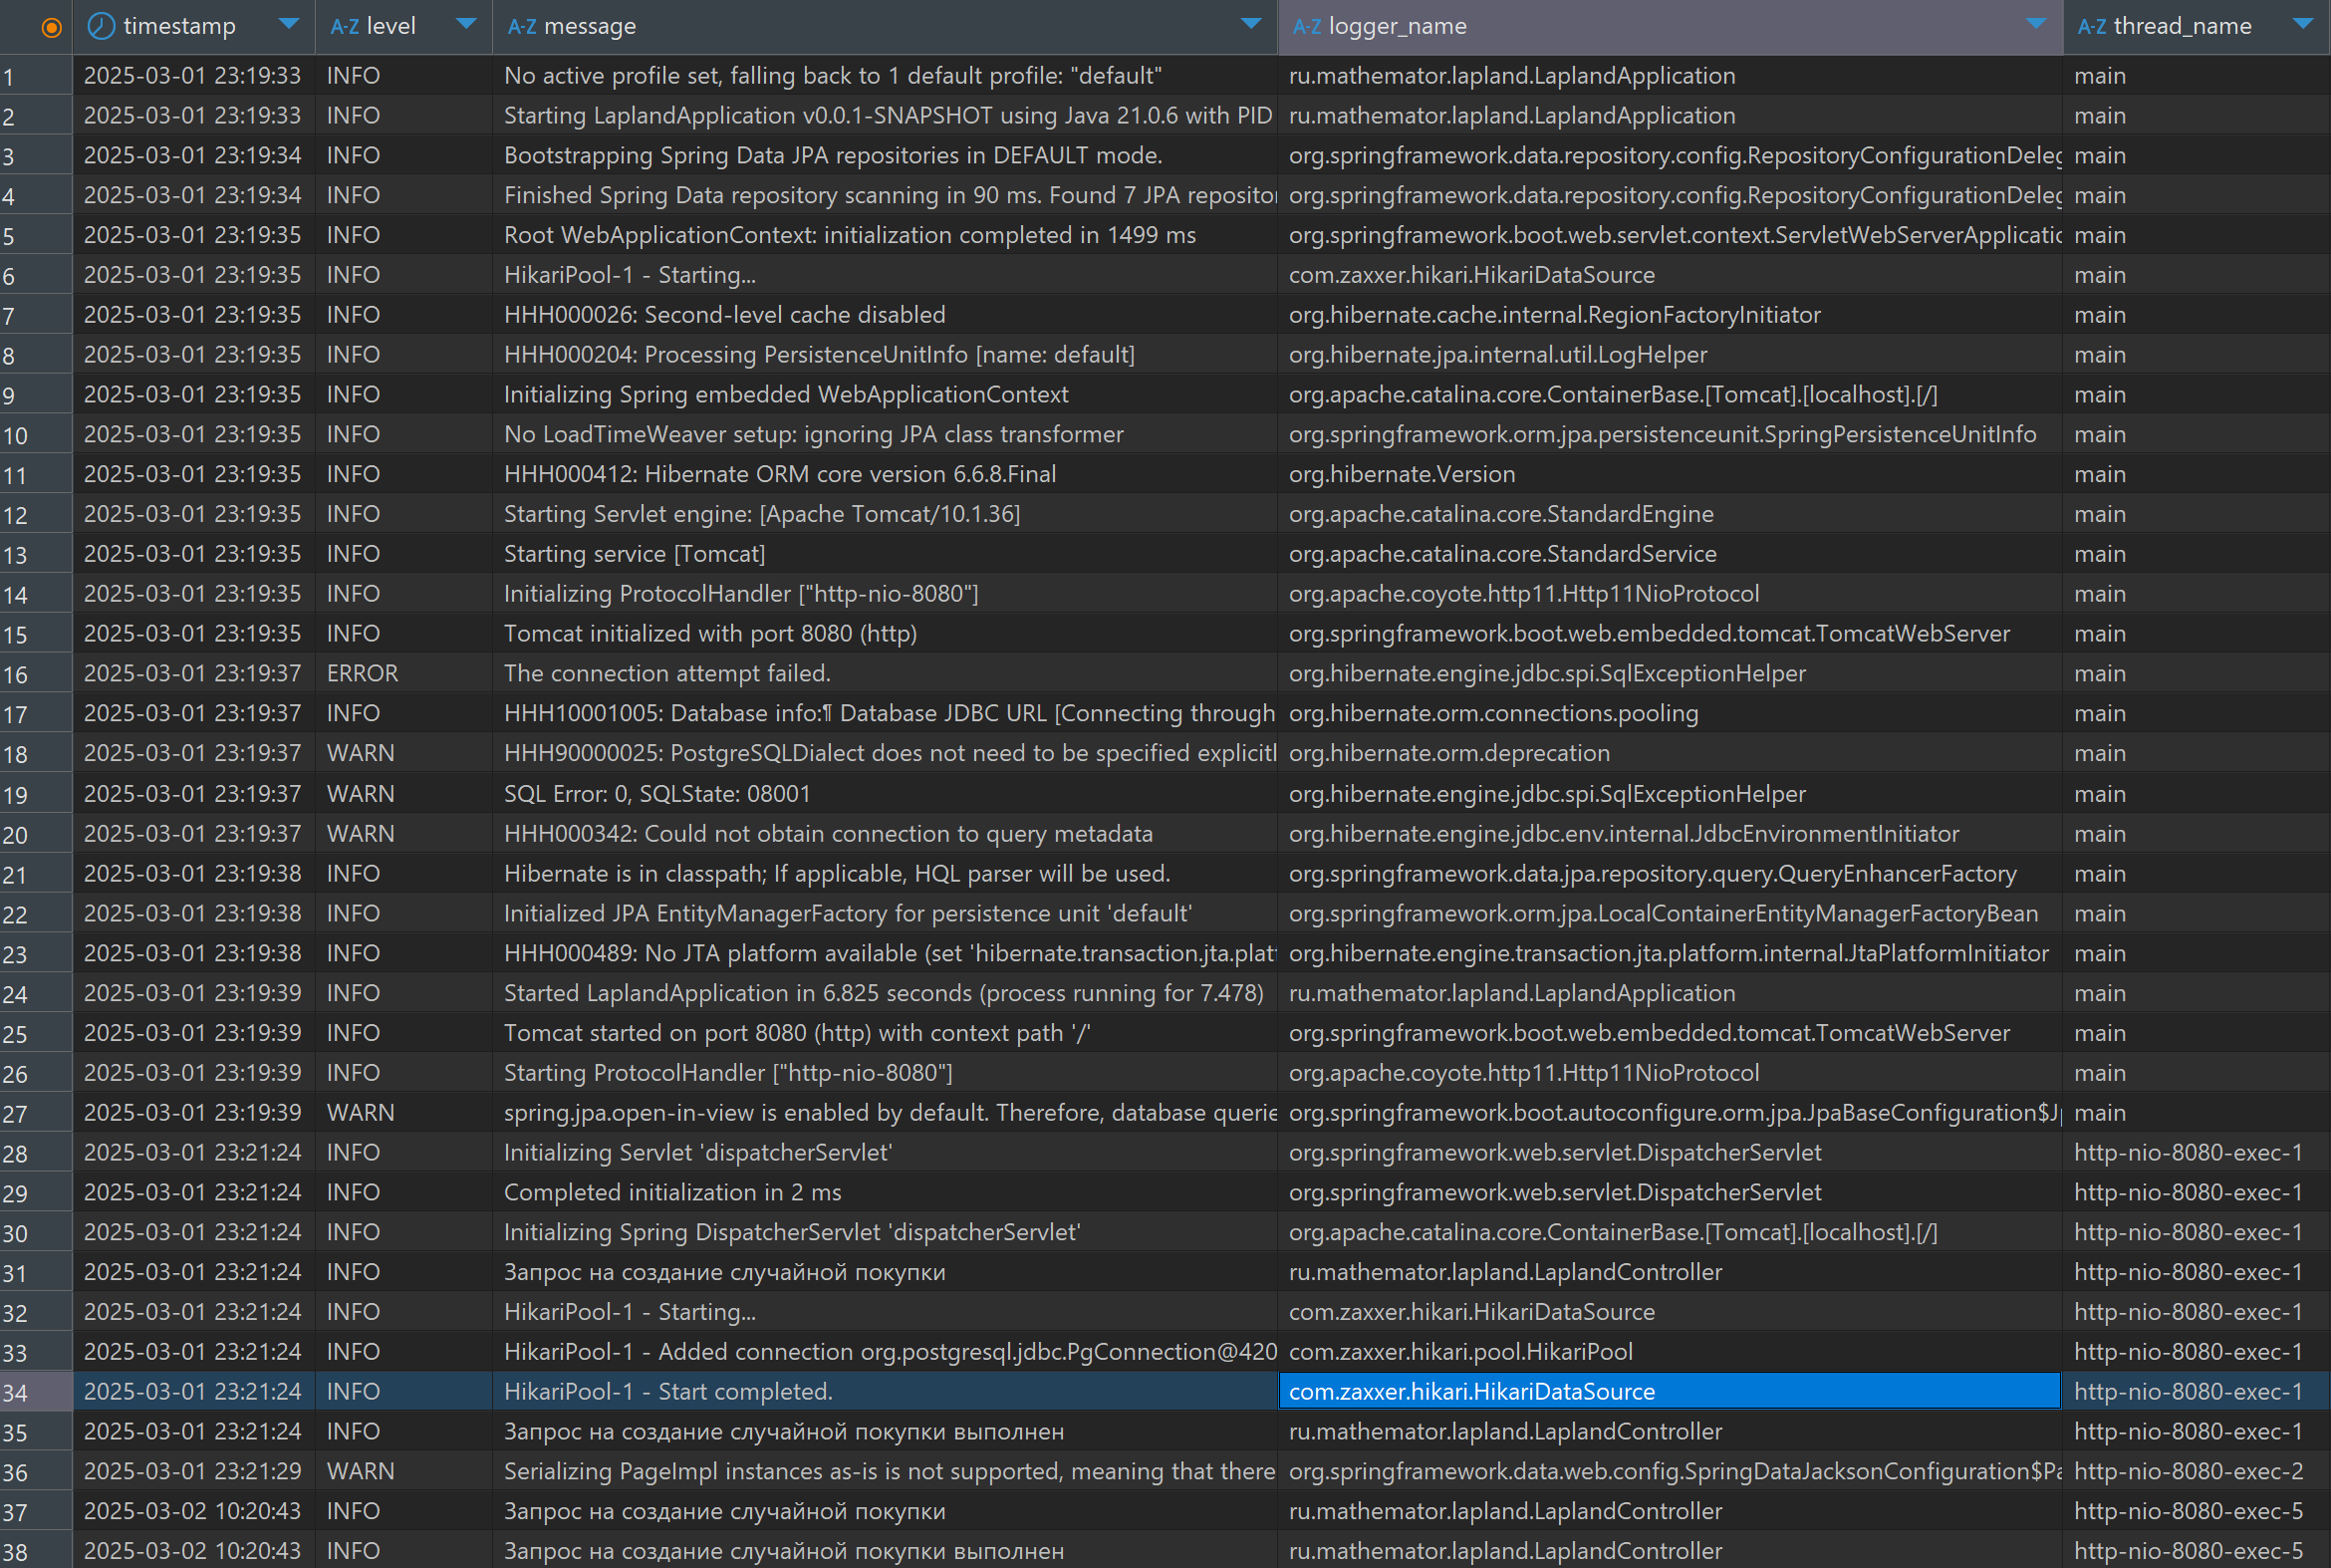
\includegraphics[width=0.9\textwidth]{clickhouse} % Вставка изображения
    \caption{Интерфейс DBeaver. Привычные логи Spring Boot приложения в таблице Clickhouse}\label{fig:clickhouse}
\end{figure}

\subsection{Нюансы настройки}\label{subsec:clickhousedetails}
В ходе развертывания решения возникла проблема в несоответствии timestamp-форматов, попадающих в Logstash и у
Clickhouse.
Для решения данной проблемы в конфигурацию был добавлен фильтр с функцией на ruby:
\begin{lstlisting}[language=ruby, frame=single, basicstyle=\normalsize\ttfamily, breaklines=true,label={lst:rubylist}]
event.set('timestamp', event.get('timestamp').time.localtime.strftime('%Y-%m-%d %H:%M:%S'))
\end{lstlisting}


